\documentclass[nochap]{config/ejercicios}

\title{Práctica CytoScape}
\author{Sandra Mingo Ramírez}
\date{2024/25}

\usepackage[all]{nowidow}
\usepackage{listing}
\usepackage{color}
\usepackage{tabularx}

\definecolor{dkgreen}{rgb}{0,0.6,0}
\definecolor{gray}{rgb}{0.5,0.5,0.5}
\definecolor{mauve}{rgb}{0.58,0,0.82}

\begin{document}
\maketitle
\tableofcontents
\newpage

%22/04 - Florencio Pazos
\section{CytoScape}
Iremos siguiendo \href{https://csbg.cnb.csic.es/pazos/cursos/UAM_Master/cytoscape_practical/}{este guion}. 

Calculando parámetros topológicos podemos obtener las métricas de redes biológicas y extraer así información de ellas. Esto se puede realizar con CytoScape. Se puede atacar la red de forma interactiva (CytoScape y programas similares), pero los cálculos masivos son algo limitados. Para atacar la red de forma programática existen librerías para manejar redes en distintos lenguajes de programación como R o Python. Por tanto, para la visualización de una red, se puede usar CytoScape, pero para obtener métricas, es mejor programando.

\section{Ficheros que se manejan}
Una red no es más que un conjunto de nodos y enlaces entre los nodos. CytoScape es capaz de leer estas redes simples y crudas, tanto en formatos específicos de red (.sif) como formatos genéricos (txt, csv). En ambos casos, la red se sube a CytoScape con Import/Export Network, no con load. Luego se puede también importar datos asociados a la red, como valores de expresión génica para los nodos, o constantes de afinidad. De nuevo, estos formatos de datos asociados se importan en CytoScape (Import/Export table). Con esto tenemos ya una red enriquecida con nodos, ramas e información. Manejando esta red, se pueden mover los nodos, calcular clusters, colorear según ciertos parámetros, etc. Cuando queremos guardar esta red enriquecida, se guarda como un fichero de sesión de CytoScape (.cys) que después se carga con Load. 

\begin{figure}[h]
\centering
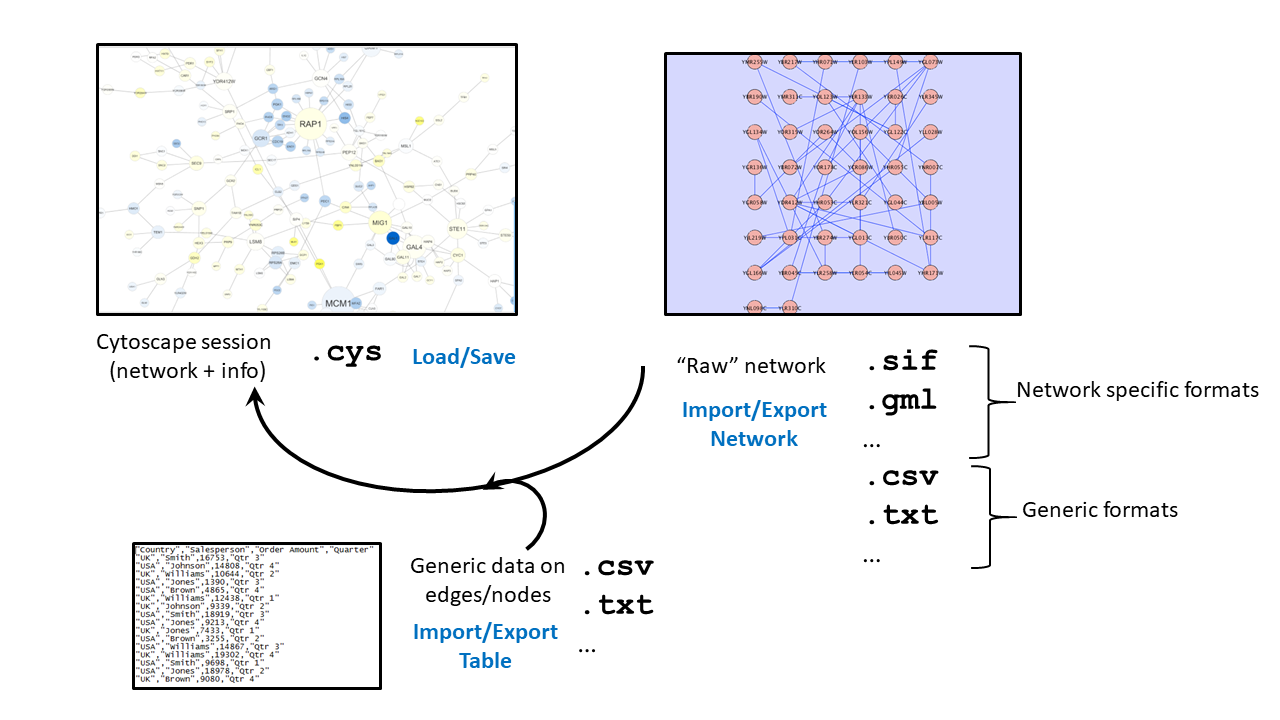
\includegraphics[width = 0.8\textwidth]{figs/cytoscape_data.png}
\end{figure}

\section{Network panels}
Para cargar una sesión de CytoScape, hay un fichero con datos genéricos. Esto se abre en File > Open Session > sampleData > galFiltered.cys.

\begin{figure}[h]
\centering
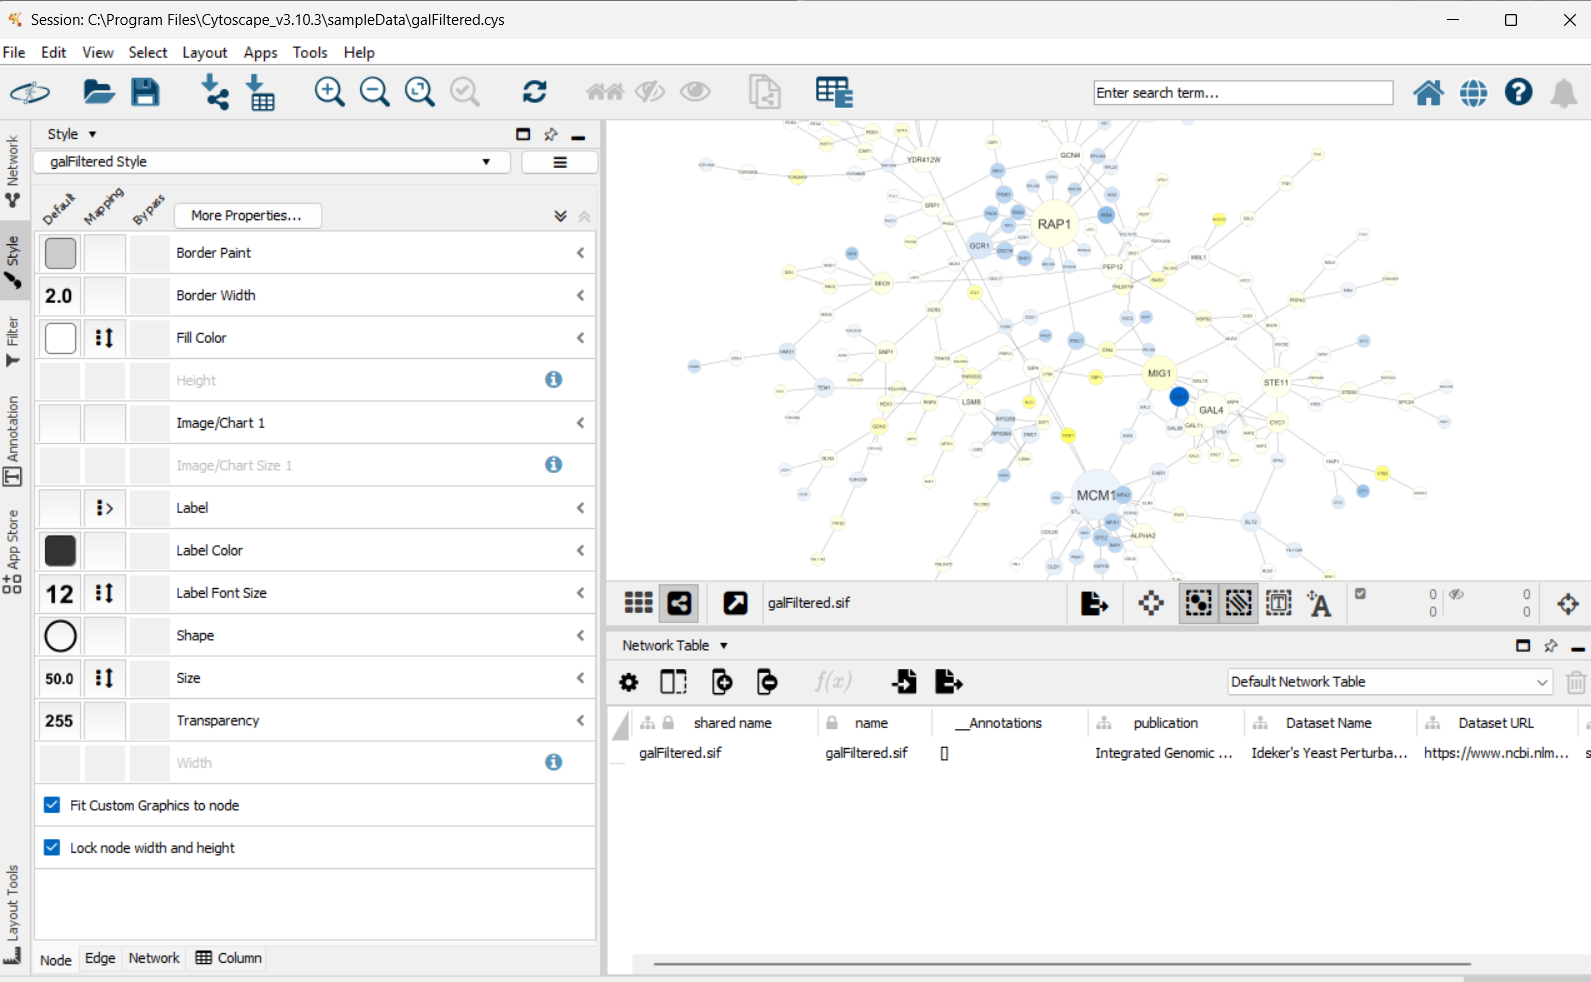
\includegraphics[width = 0.5\textwidth]{figs/sampledata.png}
\end{figure}

En el panel superior derecha se puede manejar interactivamente la red. La rueda del ratón permite hacer zoom. Moviendo fuera de la red arrastrando el ratón, se mueve la red. Esto permite ir a una región de interés y hacer zoom ahí. Al arrastrar un nodo, éste se mueve en el espacio de la red. Esto es útil para visualizar mejor una determinada región de la red. Para mover más de un nodo en conjunto, se puede arrastrar el ratón mientras se pulsa Ctrl. Así, se forma una caja, y todos los nodos que queden dentro de ella se seleccionan. La selección se deshace haciendo click fuera de la región. 

El panel inferior derecho muestra la información en formato tabular. Como solo se ha cargado una red, en la imagen solo hay una fila. No obstante, pulsando en el desplegable "Network Table" se puede seleccionar la tabla de nodos y la tabla de ramas. Si seleccionamos la tabla de nodos, se indican ciertas métricas para cada nodo, como AverageShortestPathLength, BetweennessCentrality, ClosenessCentrality, etc. Al seleccionar un nodo en el grafo, en la tabla aparece dicho nodo. Esta tabla funciona como una hoja de cálculo. De esta forma, se pueden ordenar los nodos por ejemplo por su valor de Betweenness.

En la parte superior derecha, encima del panel del grafo, hay un buscador que permite introducir el nombre de genes para que se marquen en la red. 

\section{Layouts y panel de estilos}
Un layout es una forma de disponer los nodos en una red para facilitar su visualización. Esto no cambia sus características internas y topológicas, solo la visualización, lo que facilita enfatizar distintas relaciones o jerarquías. Para aplicar distintos layouts, hay un menú en la barra superior llamado "Layout". El que está por defecto se encuentra en Prefuse Force Directed Layout > All nodes > EdgeBetweenness.

El panel de la izquierda contiene herramientas para realizar distintas acciones sobre la red. En "Style" se ven distintos estilos de visualización de la red. Un estilo no es más que un conjunto de atributos gráficos. Define el color de los nodos, su tamaño, el tipo de caracteres que se usan para el nombre, las líneas que representan las conexiones, su anchura, etc. Se pueden cargar estilos predeterminados (justo debajo del desplegable de Style) o modificar aspectos determinados en las propiedades concretas. Al modificar un estilo, se puede guardar dando a las tres líneas al lado del nombre del estilo cambiado. 

Para cambiar el estilo de un conjunto de interés, se pueden seleccionar los nodos (mediante la definición de la caja o seleccionándolos en el Data Panel) y se cambia el parámetro de estilo en la columna Bypass.

\begin{figure}[h]
\centering
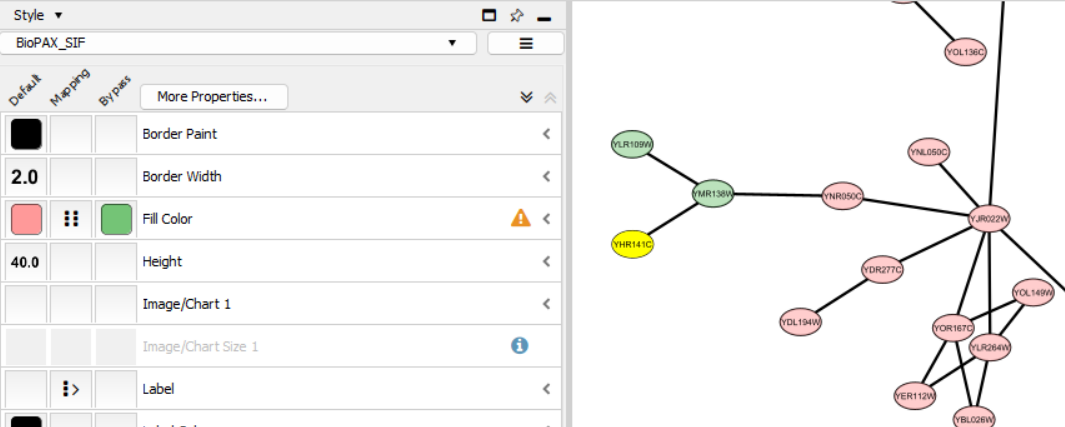
\includegraphics[width = 0.7\textwidth]{figs/style.png}
\end{figure}

\begin{figure}[h]
\centering
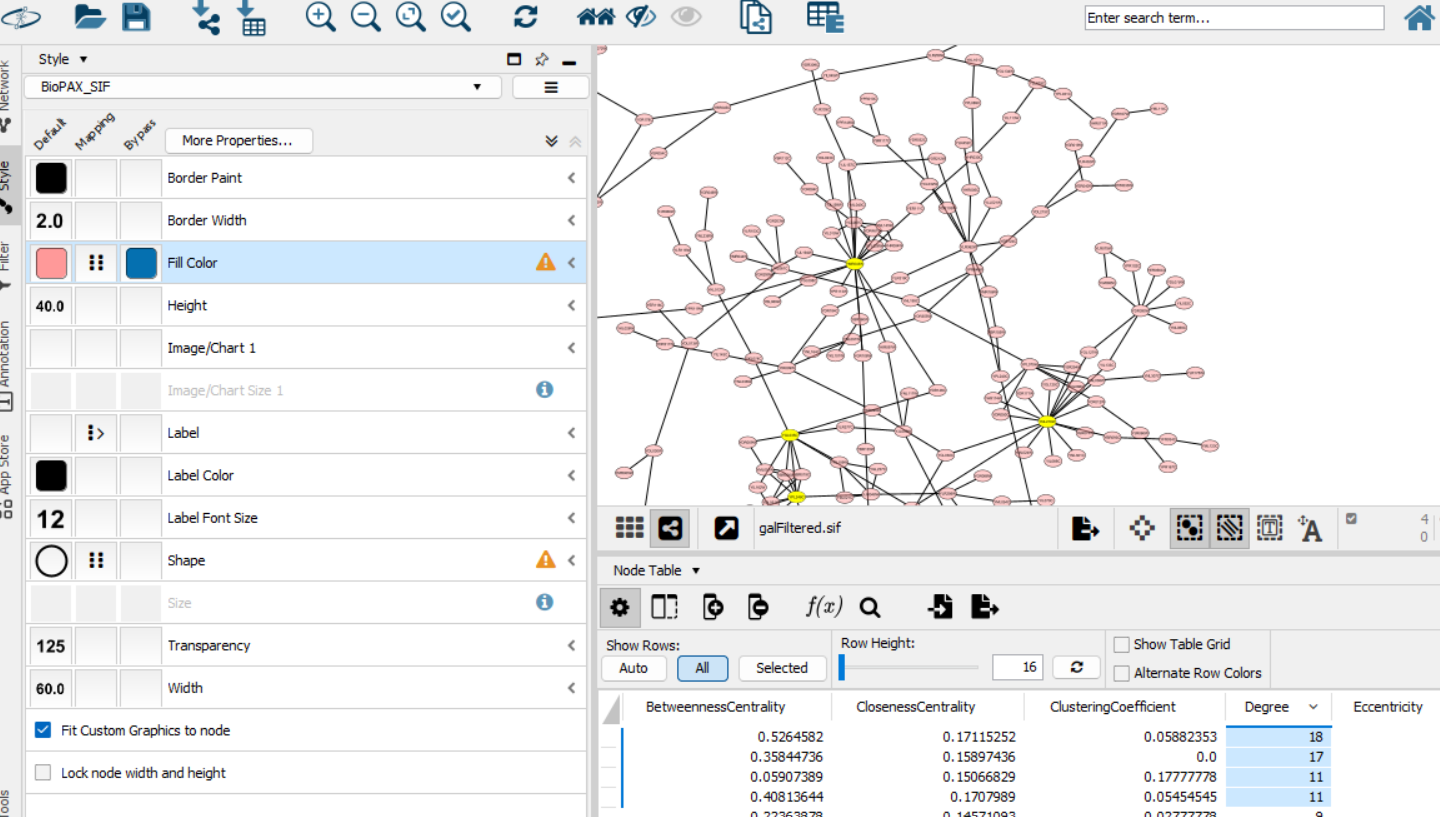
\includegraphics[width = 0.7\textwidth]{figs/style-specific.png}
\end{figure}

Hacer un mapeo es asociar un atributo gráfico a una columna. De esta forma, el atributo gráfico varía en función del valor de la métrica. Por ejemplo, queremos hacer que la anchura de las ramas sea proporcional al betweenness. Cambiamos a Edge Tables y vemos que hay una característica llamada EdgeBetweenness. Para hacer un mapeo, primero se localiza el parámetro gráfico. En este caso, queremos cambiar la anchura de las líneas, por lo que vamos primero a la pestaña de Edge (parte inferior derecha) y después a Edge. Al pulsar en la casilla de Mapping, seleccionamos un mapeo continuo.

\begin{figure}[h]
\centering
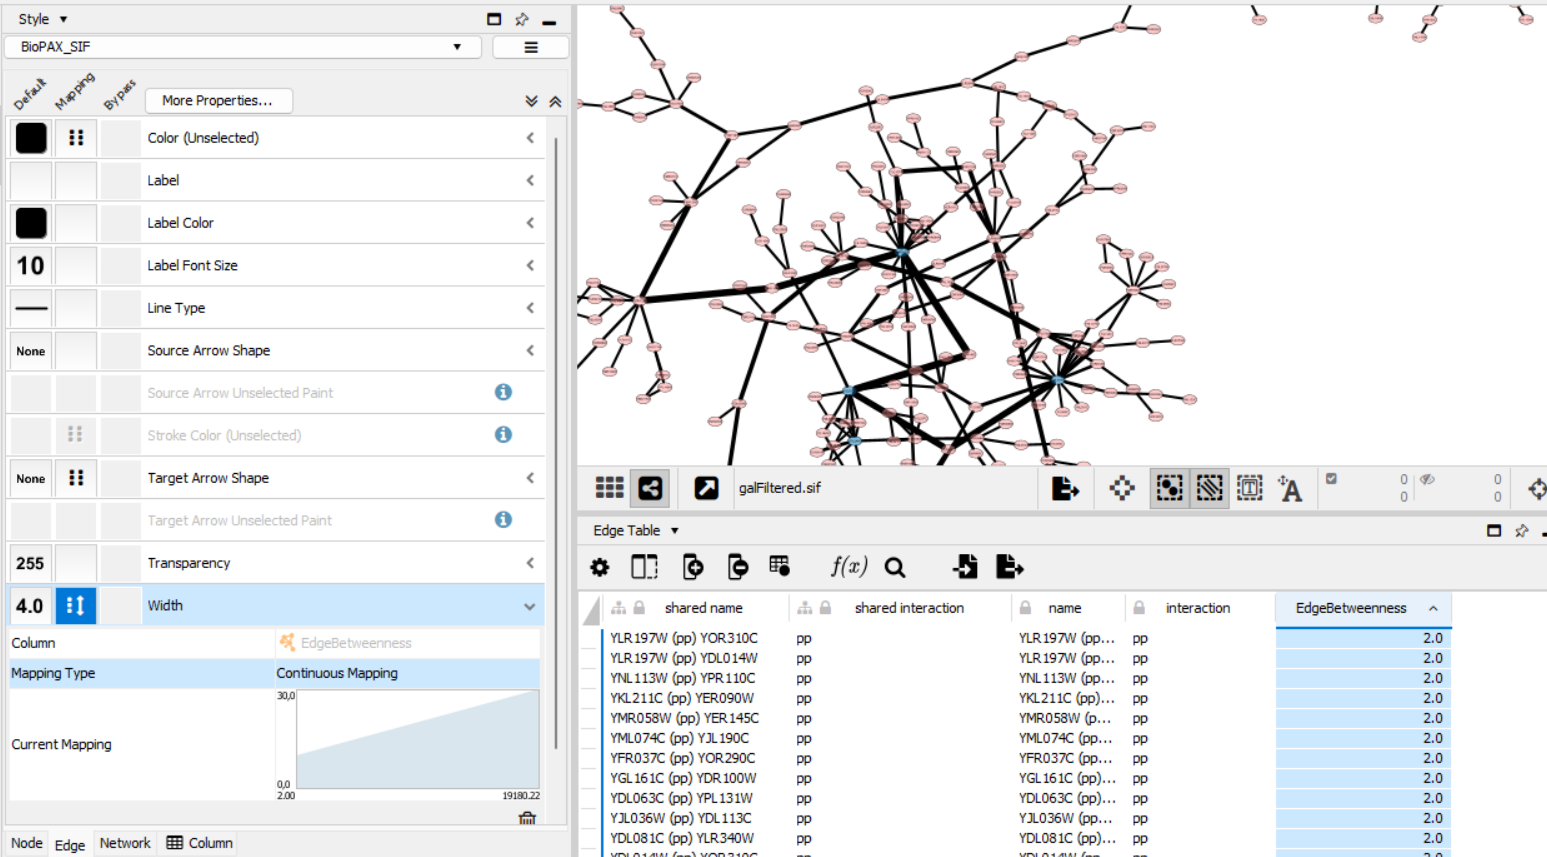
\includegraphics[width = 0.7\textwidth]{figs/style-edgewidth.png}
\end{figure}

Al hacer doble click en el gráfico de Current Mapping, se puede personalizar el grosor de las ramas según el valor.

\begin{figure}[h]
\centering
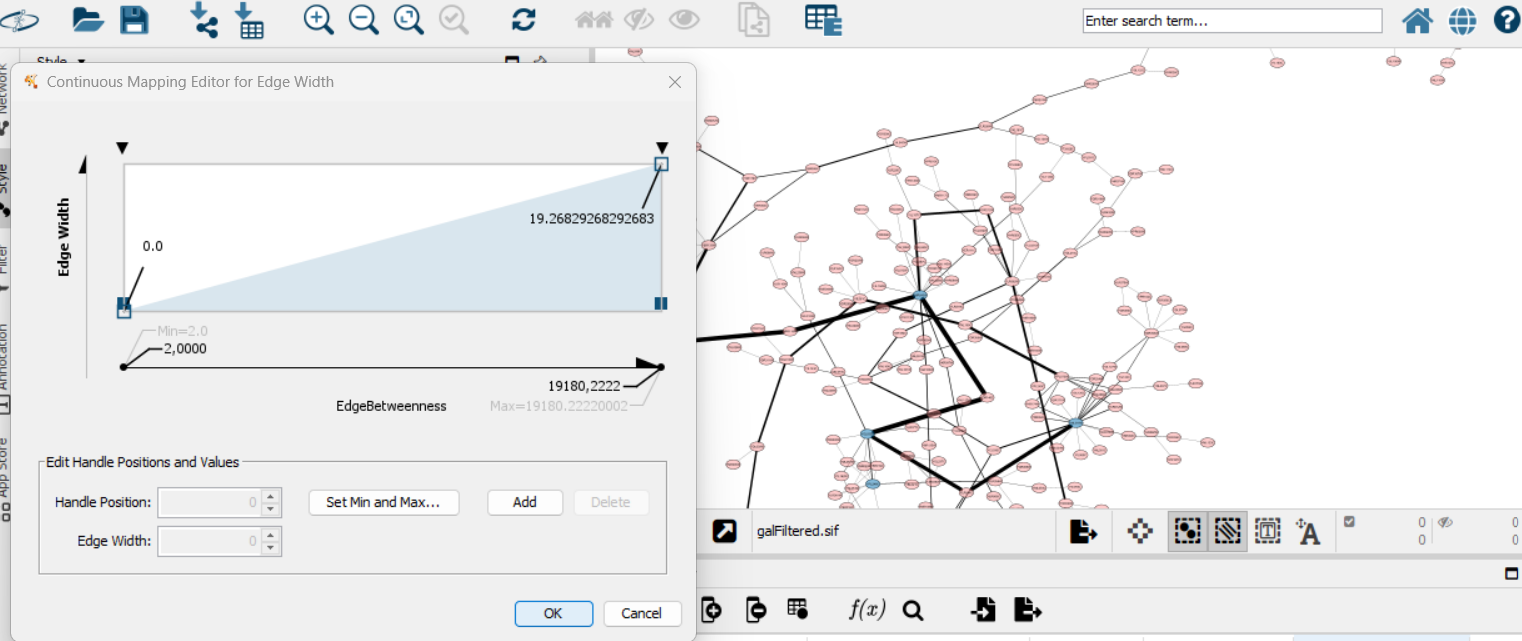
\includegraphics[width = 0.5\textwidth]{figs/style-edgewidth2.png}
\end{figure}

Esto también funciona con las características de los nodos. Volvemos a Node, y pulsamos la columna de Mapping para Fill Color. Column especificamos Degree, Continuous Mapping y se puede modificar la escala de colores, aunque ya viene por defecto un gradiente de amarillo a morado.

\begin{figure}[h]
\centering
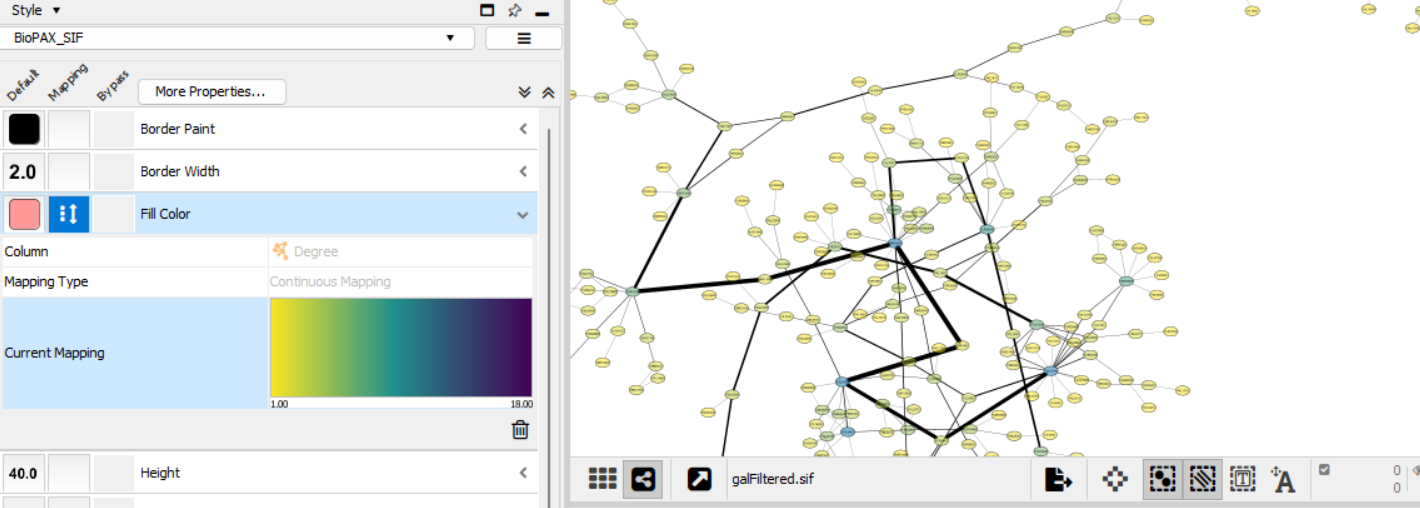
\includegraphics[width = 0.7\textwidth]{figs/style-nodefill.png}
\end{figure}

La escala de colores es compuesta. Tiene tres partes: un punto en amarillo, uno en verde y uno en morado. Se pueden mover para que la escala tenga un gradiente con más tonos en un rango o en otro. Además, se puede eliminar el punto central y cambiar los colores de los demás puntos. La escala de colores puede ser poco discriminativa, habiendo muchos nodos con un valor similar (normalmente bajo). La escala se debe adaptar a los datos, pudiendo interesar mantener el punto de color central y moverlo para que sí sea discriminativo.
Ciertos estilos bloquean algunos tipos de mapeo.

\section{Red cruda y datos adicionales}
Ahora vamos a importar una red cruda en la carpeta de sampleData. Primero File > Close Session (se puede guardar antes con File > Save Session As) y después File > Import > Network from File > importNetworkFromFile.csv. 

Como el fichero es genérico, aparece un cuadro de diálogo en el que hay que especificar qué representa cada columna. Se debe revisar que estén bien definidas con la pareja enlazada por la rama (columnas source y target). Si esas columnas no estuvieran bien identificadas, habría que pulsar "Advanced Options" y especificar el separados de columnas y otros valores. 

\begin{figure}[h]
\centering
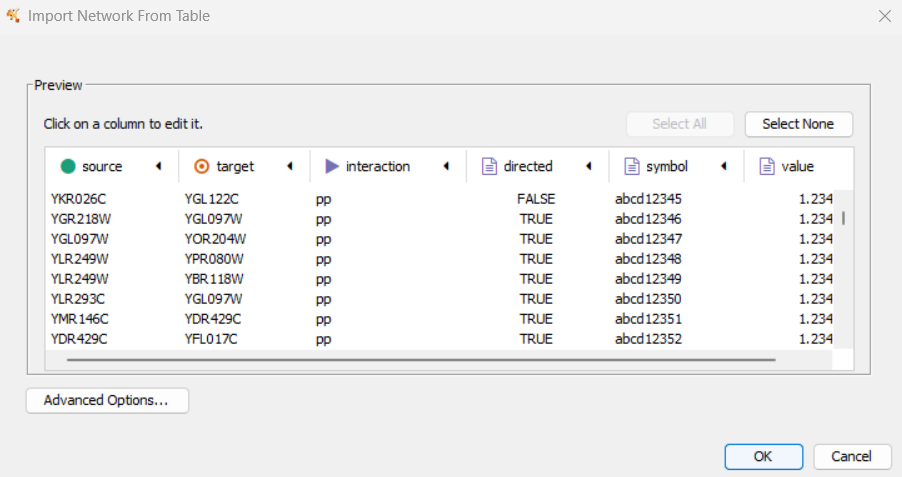
\includegraphics[width = 0.4\textwidth]{figs/importtablefromfile.png}
\end{figure}

Con la red importada, queremos importar datos adicionales. En este caso, tenemos datos de expresión asociada en un fichero llamado galExpData.csv, y lo queremos importar. File > Import > Table from File > fichero. Vuelve a aparecer un cuadro de diálogo con la cabecera, separador, etc. Lo importante es la columna con la llave, ya que es aquella que se utilizará para enlazar estos datos nuevos con la red cargada. 

\begin{figure}[h]
\centering
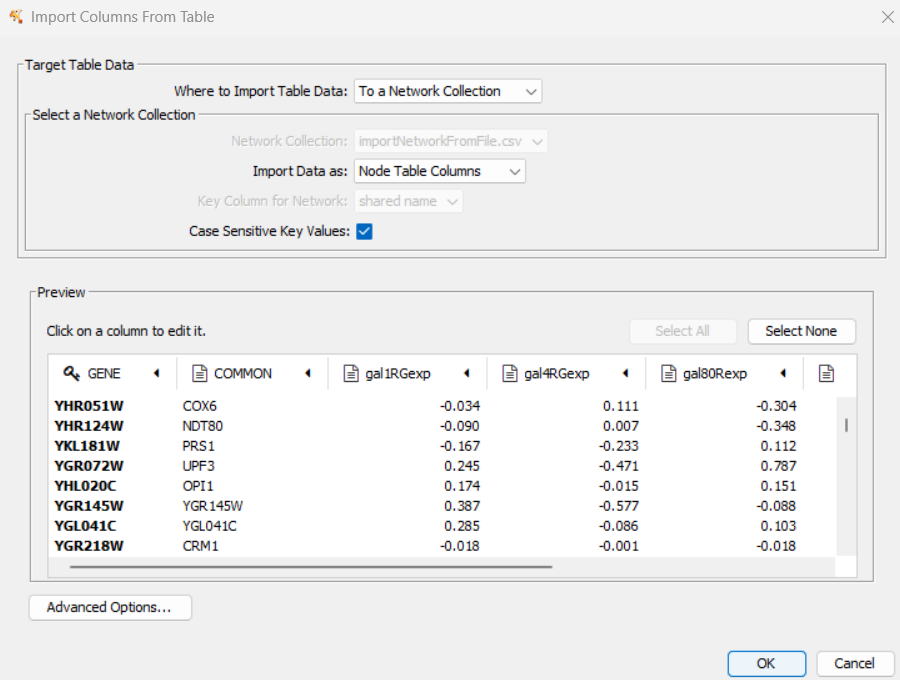
\includegraphics[width = 0.4\textwidth]{figs/importcolumnsfromtable.png}
\end{figure}

La interacción puede ser pp (proteína-proteína) o pd (proteína-ADN; control transcripcional), por lo que se puede modificar para que las conexiones pp sean con una línea punteada y pd continua. Esto se hace en Edge > Mapping Line Type y seleccionar la columna interaction, mapeo discreto y cambiar el estilo de línea.

\begin{figure}[h]
\centering
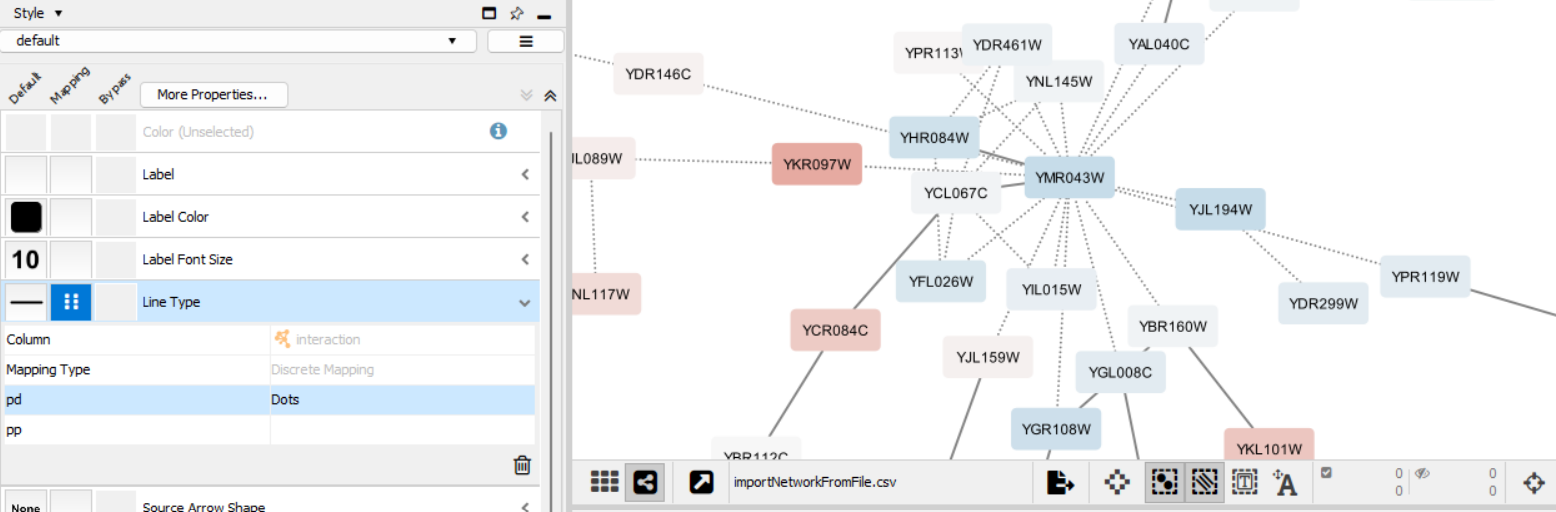
\includegraphics[width = 0.7\textwidth]{figs/style-edgeline.png}
\end{figure}

\subsection{Valores topológicos de la red}
CytoScape no es el mejor programa para calcular los parámetros de las topologías de red. Aun así, se pueden calcular. 

En Tools, hay una opción llamada Analyze Network. Al darle, primero se debe indicar si se analiza como un grafo dirigido. Asumimos en este ejemplo que no es dirigido. 

Como la red es pequeña, tarda poco en cargar. En el Data Panel han aparecido nuevas columnas con los valores topológicos de cada nodo y cada rama. 

\section{Plugins}
CytoScape es un programa al que es fácil añadir nuevas funcionalidades mediante plugins, sobre todo programando en Java. Hay muchos plugins ya desarrolladas, que en las últimas versiones han pasado a llamarse "Apps". En la barra superior Apps > App Store > Open y se pueden ver las distintas apps disponibles. Si por ejemplo quisiéramos trabajar con datos de expresión, en el buscador se puede poner "expression" y aparecen apps que añaden funcionalidades para trabajar con estos datos de expresión.

\end{document}